\chapter{Design Methodology}
\label{ch:design_methodology}

% \section{Overview}
This chapter formulates the system model for identification-based synchronization and derives the theoretical bounds for its reliability and latency. We contrast the data flow of classical transmission with the proposed identification scheme, explicitly breaking down the operational stages from state generation to synchronization. We then quantify the collision probabilities and end-to-end latency based on these distinct workflows.

\section{System Model and Data Flow}
\label{sec:system_model}

We consider a networked control system where a Robot (Sender) synchronizes its state $S_t$ with a Digital Twin (Receiver) maintaining a prediction $\hat{S}_t$. The fundamental difference between the two approaches lies in their data processing pipelines.

\subsection{Baseline: Traditional Transmission Flow}
The standard synchronization protocol follows a linear, ``always-on'' approach. As illustrated in Figure~\ref{fig:trad_flow}, the data flow consists of three sequential stages:

\begin{figure}[htbp]
    \centering
    % Ensure you have the file 'figures/trad.png'
    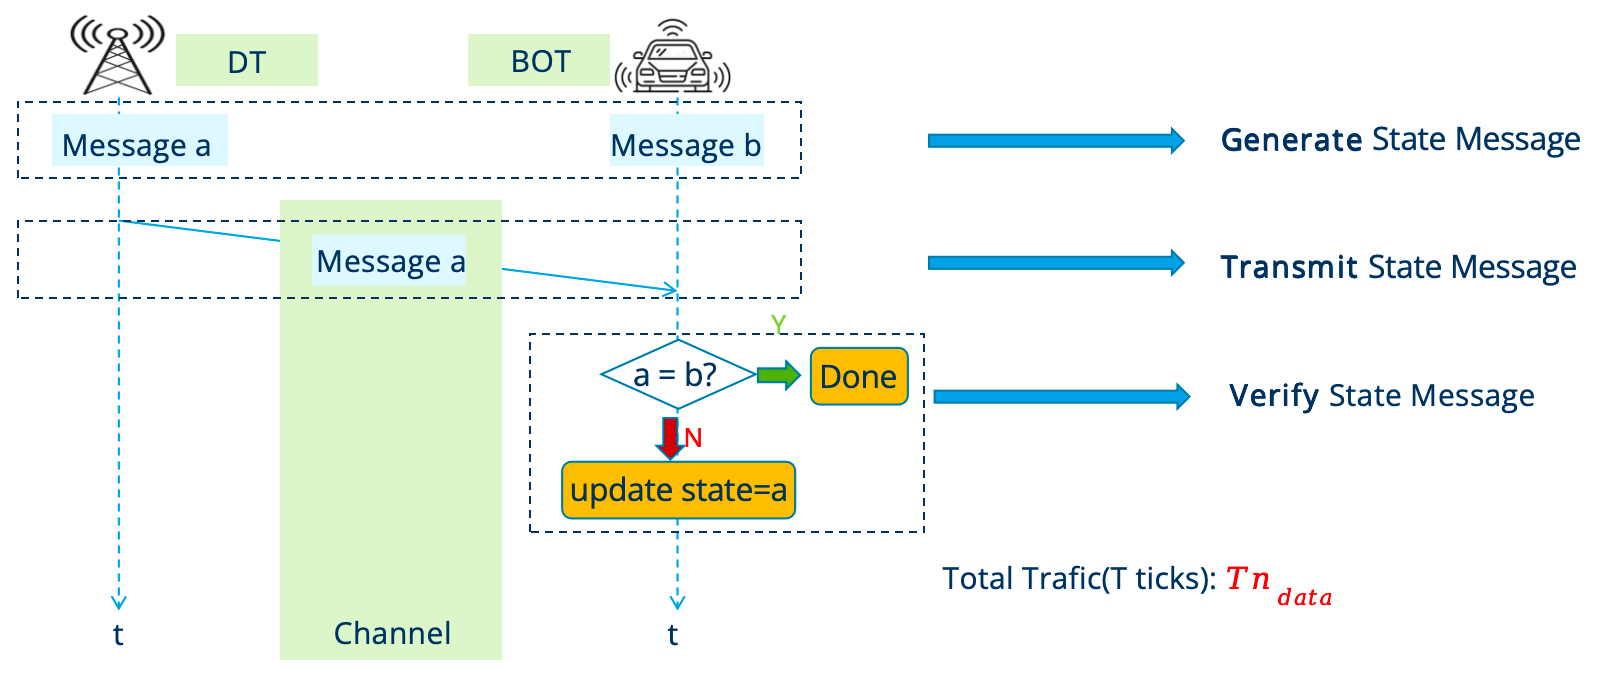
\includegraphics[width=0.8\textwidth]{figures/trad.png}
    \caption{Data flow of Traditional Synchronization: The full state is transmitted regardless of the Digital Twin's knowledge.}
    \label{fig:trad_flow}
\end{figure}

\begin{enumerate}
    \item \textbf{Generate:} The robot samples its sensors to generate the full state message $S_t$ of size $n_{data}$.
    \item \textbf{Transmit:} The entire payload $S_t$ is transmitted over the channel. This step consumes bandwidth proportional to the state dimension, regardless of whether $S_t$ has changed significantly or matches the DT's prediction.
    \item \textbf{Verify/Update:} The DT receives the message, overwrites its local prediction $\hat{S}_t$ with the received $S_t$, and confirms the update.
\end{enumerate}
This process is robust but inefficient, as the \textbf{Transmit} stage imposes a heavy, constant latency penalty ($T_{trans} = n_{data}/B$).

\subsection{Proposed: Identification (ID) Data Flow}
The identification-based protocol introduces computational intelligence to reduce communication load. As shown in Figure~\ref{fig:id_flow}, the pipeline is expanded to five stages, introducing a ``Verify-then-Correct'' logic:

\begin{figure}[htbp]
    \centering
    % Ensure you have the file 'figures/ID.png'
    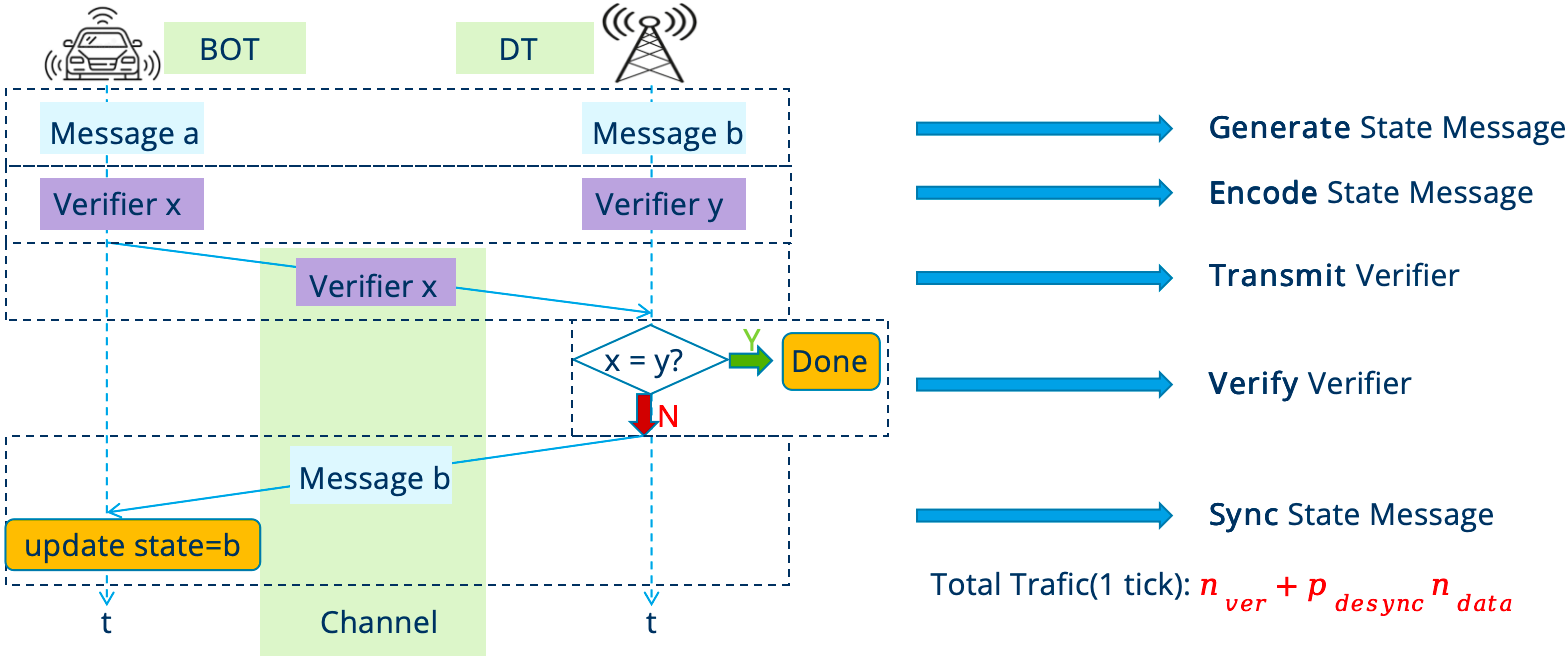
\includegraphics[width=0.8\textwidth]{figures/ID.png}
    \caption{Data flow of ID Synchronization: High-bandwidth transmission is replaced by local encoding and conditional fallback.}
    \label{fig:id_flow}
\end{figure}

\begin{enumerate}
    \item \textbf{Generate:} Both the Robot and the DT independently generate their respective state views: the actual state $S_t$ and the predicted state $\hat{S}_t$.
    \item \textbf{Encode:} Instead of preparing the full message for transmission, the Robot computes a compact signature (verifier) $v = E(S_t, r)$ using a shared seed $r$. Simultaneously, the DT computes its local reference $\hat{v} = E(\hat{S}_t, r)$. This step introduces a computational latency ($t_{ver}$) but drastically compresses the data.
    \item \textbf{Transmit:} Only the short verifier $v$ (size $n_{ver} \ll n_{data}$) is sent over the channel.
    \item \textbf{Verify:} The DT compares the received $v$ with its local $\hat{v}$.
    \item \textbf{Sync (Conditional):} 
    \begin{itemize}
        \item If $v = \hat{v}$, the process terminates (Done).
        \item If $v \neq \hat{v}$, a mismatch is detected. The system enters a fallback mode, requesting the full transmission of $S_t$ to resynchronize.
    \end{itemize}
\end{enumerate}

\section{Encoding Mechanisms and Reliability Analysis}
\label{sec:reliability_analysis}

The safety of the ID flow depends on the reliability of the \textbf{Verify} stage. A critical failure occurs if the states differ ($S_t \neq \hat{S}_t$) but their verifiers collide ($v = \hat{v}$), defined as a Type II Error ($p_{miss}$). We investigate two distinct encoding mechanisms, detailing their construction and theoretical error bounds.

\subsection{Algebraic Construction and Error Analysis (RS-ID)}
\label{sec:rsid_proof}

The core challenge of the RS-ID scheme is to map a high-dimensional state vector $S$ of length $n_{data}$ into a single element within a finite field $\mathbb{F}_q$, where the field size $q = 2^{n_{ver}}$ is determined by the output bandwidth constraint.

\textbf{Polynomial Construction (The ``Chunking'' Process)}
Since the operations are defined over $\mathbb{F}_{q}$, a state vector $S$ typically exceeds the capacity of a single field element (i.e., $n_{data} \gg n_{ver}$). To resolve this dimensionality mismatch, we decompose the bitstream $S$ into $k$ segments, where each segment represents a coefficient in the field:
\begin{equation}
    k = \left\lceil \frac{n_{data}}{n_{ver}} \right\rceil
\end{equation}
Let $S$ be represented as a vector of coefficients $\{s_0, s_1, \dots, s_{k-1}\}$, where each $s_i \in \mathbb{F}_q$. We then construct a polynomial $P_S(x)$ of degree at most $k-1$:
\begin{equation}
    P_S(x) = \sum_{i=0}^{k-1} s_i x^i
\end{equation}
The verifier $v$ is obtained by evaluating this polynomial at a shared random seed $r$: $v = P_S(r)$.

\textbf{Proof of Collision Probability}
A Type II error (Miss) occurs when the Digital Twin predicts an incorrect state $\hat{S} \neq S$, yet the generated verifiers are identical ($P_{\hat{S}}(r) = P_S(r)$).
We define a \textit{difference polynomial} $\Delta(x)$:
\begin{equation}
    \Delta(x) = P_S(x) - P_{\hat{S}}(x)
\end{equation}
Since $S \neq \hat{S}$, at least one coefficient differs, making $\Delta(x)$ a non-zero polynomial with a degree $\text{deg}(\Delta) \leq k-1$.
A collision event is mathematically equivalent to finding a root of this difference polynomial: $\Delta(r) = 0$.

We invoke the \textbf{Schwartz-Zippel Lemma} (Lemma 1 in~\cite{schwartz1980fast}), which states that a non-zero polynomial of degree $d$ over a field $\mathbb{F}_q$ has at most $d$ roots.
Mapping this theorem to our system parameters:
\begin{itemize}
    \item The polynomial degree $d$ corresponds to the chunk count $k \approx n_{data}/n_{ver}$.
    \item The sample space size corresponds to the field size $q = 2^{n_{ver}}$.
\end{itemize}
Consequently, for a uniformly distributed random seed $r$, the probability of collision is bounded by:
\begin{equation}
    P_{miss}^{RS} = \Pr[\Delta(r) = 0] \leq \frac{\text{deg}(\Delta)}{q} < \frac{k}{2^{n_{ver}}} = \frac{\lceil n_{data}/n_{ver} \rceil}{2^{n_{ver}}}
    \label{eq:rsid_bound}
\end{equation}

\textbf{Theoretical Implication}
This derivation highlights the structural trade-off in algebraic identification. The term $k$ in the numerator represents the complexity of the data: as the data size $n_{data}$ grows, the polynomial becomes more complex (higher degree), increasing the number of potential roots (collisions). Therefore, to maintain a constant safety margin $P_{miss}$, the verifier length $n_{ver}$ must scale logarithmically with the data size.

\subsection{Cryptographic Construction and Error Analysis (SHA-256)}
\label{sec:sha256_proof}

Unlike the algebraic structure of RS-ID, the security of hash-based identification relies on computational hardness assumptions. We verify the state using a truncated cryptographic hash function (SHA-256):
\begin{equation}
    v = \text{Truncate}(\text{SHA-256}(S || r), n_{ver})
\end{equation}
where $||$ denotes concatenation with the random seed $r$.

\textbf{Random Oracle Assumption}
To analyze the collision probability theoretically, we adopt the \textbf{Random Oracle Model (ROM)} paradigm introduced by Bellare and Rogaway~\cite{bellare1993random}. In this model, the hash function $H(\cdot)$ is idealized as a mathematical oracle that maps every unique input query to a response selected \textbf{uniformly and independently} from the output domain $\{0, 1\}^{n_{ver}}$.

\textbf{Proof of Collision Probability (Derivation from Uniformity)}
Under the ROM, for any robot state $S$, the hash output $H(S||r)$ is a random variable following a uniform distribution over the verifier space of size $N = 2^{n_{ver}}$.
Given a pre-calculated verifier $\hat{v}$ from the Digital Twin, the probability of a collision (Type II error) is equivalent to the probability that a uniformly selected random value hits a specific target in the sample space.
\begin{equation}
    P_{miss}^{SHA} = \Pr[H(S||r) = \hat{v}] = \frac{1}{|\{0, 1\}^{n_{ver}}|} = \frac{1}{2^{n_{ver}}}
    \label{eq:sha_bound}
\end{equation}
This derivation relies on the property that in a uniform distribution, the probability of any single outcome is the reciprocal of the sample space size.

\textbf{Comparative Analysis: RS-ID vs. SHA-256}
A critical distinction arises when comparing this bound with Equation~\eqref{eq:rsid_bound} (the RS-ID bound).
\begin{itemize}
    \item \textbf{RS-ID Dependency:} The error probability in RS-ID scales linearly with the data size ($k \approx n_{data}/n_{ver}$), reflecting the geometric constraint that higher-degree polynomials have more roots.
    \item \textbf{SHA-256 Independence:} In contrast, under the Random Oracle assumption, the error probability for SHA-256 is \textbf{invariant} to the input data size $n_{data}$.
\end{itemize}
This property makes the cryptographic approach structurally more robust for large-scale state vectors (e.g., LiDAR point clouds), as the ``collision risk'' does not accumulate with data length. However, this comes at the cost of losing the unconditional algebraic guarantee provided by the Schwartz-Zippel Lemma, replacing it with a computational assumption.

\subsection{Tolerance-Based Verification (K-ID)}
\label{sec:kid_model}
The ID data flow described in Section~\ref{sec:system_model} assumes a strict equality check between a single predicted state $\hat{S}_t$ and the true state $S_t$. In practice, however, many cyber-physical systems can tolerate bounded deviations without requiring a full resynchronization. We therefore extend the verification stage to a \textit{tolerance-based} rule, referred to as \textbf{K-ID}.

\textbf{Acceptable Set:}
Given the DT prediction $\hat{S}_t$ and a tolerance radius $K$, the DT defines an acceptable set
\begin{equation}
    \mathcal{A}_K(\hat{S}_t)=\{s\mid \lVert s-\hat{S}_t\rVert\le K\}.
\end{equation}
In the experiments in this thesis, we use a scalar state for clarity (so $\lVert\cdot\rVert$ is absolute value), but the K-ID logic generalizes to vector-valued states with an appropriate norm.

\textbf{K-ID Decision Rule:}
The Robot sends a truncated hash verifier
\begin{equation}
    v=\mathrm{Truncate}(\mathrm{SHA256}(S_t\Vert r),n_{ver}).
\end{equation}
The DT pre-computes the set of valid verifiers for the acceptable states,
\begin{equation}
    \mathcal{V}_K=\{\mathrm{Truncate}(\mathrm{SHA256}(s\Vert r),n_{ver})\mid s\in \mathcal{A}_K(\hat{S}_t)\},
\end{equation}
and \textit{accepts} if $v\in\mathcal{V}_K$. Otherwise, it triggers fallback and requests the full payload.

\textbf{Safety Miss Rate:}
Define an \textit{unsafe} event as the true state lying outside the tolerance region, i.e., $S_t\notin\mathcal{A}_K(\hat{S}_t)$. A miss occurs when the DT accepts despite being unsafe:
\begin{equation}
    p_{miss,K}=\Pr[\,v\in\mathcal{V}_K\mid S_t\notin\mathcal{A}_K(\hat{S}_t)\,].
\end{equation}
Under the Random Oracle assumption used in Section~\ref{sec:sha256_proof}, the verifier $v$ for an unsafe state is uniform over $\{0,1\}^{n_{ver}}$. Hence, the conditional miss probability is bounded by the fraction of verifier space covered by acceptable hashes:
\begin{equation}
    p_{miss,K}^{SHA}\approx \frac{|\mathcal{V}_K|}{2^{n_{ver}}} \le \frac{|\mathcal{A}_K(\hat{S}_t)|}{2^{n_{ver}}}.
    \label{eq:kid_sha_bound}
\end{equation}
This highlights a key trade-off: increasing $K$ enlarges the acceptable set (reducing fallback frequency), but also increases the miss probability conditional on being unsafe.

\textbf{Unsafe Rate and Latency:}
Let $p_{unsafe}(K)=\Pr[S_t\notin\mathcal{A}_K(\hat{S}_t)]$. If the prediction error $e=S_t-\hat{S}_t$ is modeled as $\mathcal{N}(0,\sigma^2)$, then
\begin{equation}
    p_{unsafe}(K)=\Pr[|e|>K]=2\bigl(1-\Phi(K/\sigma)\bigr).
\end{equation}
Since fallback is triggered when the DT is unsafe and \emph{does not} miss, the expected latency follows the same structure as Section~\ref{sec:latency_model} but with the tolerance-aware terms:
\begin{equation}
    T_{KID} = t_{ver} + \frac{n_{ver}}{B} + p_{unsafe}(K)\bigl(1-p_{miss,K}\bigr)\frac{n_{data}}{B}.
    \label{eq:kid_latency}
\end{equation}
The empirical sweep in Chapter~\ref{ch:results} instantiates this model and visualizes the safety--latency trade-off across $K$ and $n_{ver}$.

\section{End-to-End Latency Model}
\label{sec:latency_model}

Based on the data flows defined in Section~\ref{sec:system_model}, we mathematically formulate the expected latency.

\textbf{Traditional Latency ($T_{trad}$):}
Since the traditional flow always executes the full transmission, its latency is deterministic:
\begin{equation}
    T_{trad} = \frac{n_{data}}{B}
\end{equation}
where $B$ is the channel bandwidth.

\textbf{Identification Latency ($T_{ID}$):}
The ID flow is probabilistic. The total time includes the mandatory encoding and verifier transmission, plus the conditional penalty for fallback. Matching the stages in Figure~\ref{fig:id_flow}:
\begin{equation}
    T_{ID} = \underbrace{t_{ver}}_{\text{Encode}} + \underbrace{\frac{n_{ver}}{B}}_{\text{Transmit Verifier}} + \underbrace{p_{desync}(1 - p_{miss}) \frac{n_{data}}{B}}_{\text{Sync (Fallback Penalty)}}
\end{equation}

\begin{itemize}
    \item $t_{ver}$: The computational time for the \textbf{Encode} stage.
    \item $p_{desync}$: The probability that the DT's prediction fails ($S_t \neq \hat{S}_t$).
    \item $(1 - p_{miss}) \frac{n_{data}}{B}$: The penalty is incurred only when a desynchronization exists AND is successfully detected by the verifier check.
\end{itemize}

This model highlights the fundamental trade-off: ID reduces the transmission term from $\frac{n_{data}}{B}$ to $\frac{n_{ver}}{B}$ but adds a computational cost $t_{ver}$. Therefore, ID is advantageous only when the bandwidth $B$ is limited (making transmission expensive) or when the prediction accuracy is high (keeping $p_{desync}$ small).